\documentclass[11pt,a4paper,polish,thesis]{dcsbook}

\usepackage[T1]{fontenc}
\usepackage[utf8]{inputenc}
\usepackage{babel}
\usepackage{graphicx}

\setcounter{secnumdepth}{3}
\setcounter{tocdepth}{3}

\begin{document}

\author{Patryk Dąbrowski 100584\\ Aleksander Kędzierski 98875\\ Paweł Lampe 99277\\ Mateusz Sikora 99615}
\title{Platforma zarządzania zdarzeniami na urządzeniach mobilnych if\{y\}}
\supervisor{dr inż.~Jerzy Błaszczyński}
\date{Poznań, 2014}

\maketitle

\frontmatter

\tableofcontents{}

\mainmatter

\chapter{Wstęp}
%% Bardzo suchy wstęp zawierający to co ma być zawarte w klasycznym wstępie pracy inżynierskiej
\section{Opis problemu i koncepcja jego rozwiązania (motywacja?)}
Współczesne urządzenia mobilne dysponują ogromnym zbiorem możliwości. Nie są to już tylko telefony które dawniej służyły wyłącznie do komunikacji. Obecnie rynek pełen
jest urządzeń z zakresu; od tabletu do smartfonu. Mnogość typów urządzeń oraz tendencja do upodabniania się między sobą uniemożliwia jednoznaczne stwierdzenie do
czego właściwie służą.

Nie lepiej sytuacja ma się w przypadku programistów piszących aplikacje na urządzenia mobilne. Nie dość, że niemal każde urządzenie ma inny osprzęt, to co więcej, na
rynku figuruje kilka wiodących mobilnych systemów operacyjnych. Wszystko to wpływa dość drastycznie na charakter rynku aplikacji mobilnych. W większej części są to
proste aplikacje realizujące bardzo ściśle określone usługi. Prowadzi to do sytuacji, w której na przeciętnym smartfonie trzeba mieć 10-20 aplikacji które pozwolą osiągnąć stabilny poziom zadowolenia.

Gdyby istniała otwartoźródłowa aplikacja pozwalająca na stosunkowo prosty dostęp do możliwości telefonu oraz ułatwiająca proces programowania, wiele małych aplikacji
mogło by stać się prostymi receptami instruującymi aplikację--matkę jak wykonać stosunkowo proste zadania. W tym przypadku 10-20 małych aplikacji można by zamienić
na jedną zawierającą w środku 10-20 prostych kawałków kodu którymi można w pełni zarządzać.

Taka aplikacja oczywiście nie istnieje. Istnieją podobne, mniej lub bardziej udane rozwiązania. Wszystkie jednak są komercyjne co jest kluczową wadą. Zamkniętość kodu
-- bo o tym tutaj mowa, ogranicza zbiór osób zaangażowanych w tworzene i pielengnację kodu. Ma to ogromne implikacje na rozwój aplikacji, co z kolei uderza w jej
użytkowników. W przypadku jakiegokolwiek złożonego problemu, użytkownik nie jest w stanie samemu sprawdzić czy problem leży po stronie jego kodu, czy po
stronie kodu aplikacji.

Skoro wyżej wspomniana, otwartoźródłowa aplikacja nie istnieje, warto by ją stworzyć. Unicestwiło by to wszystkie wspomniane powyżej problemy. Taka też idea leży u
podstaw tej pracy. Stworzyć wolną, otwartoźródłową aplikację służącom przeciętnym użytkownikom. Co jednak nawet ważniejsze, stworzyć kod, który będzie mógł zostać
użyty przez zaawansowanych użytkowników-programistów.

\section{Cele i zakres pracy}
Postawowym celem niniejszej pracy, jest stworzenie otwartoźródłowej biblioteki uproszczającej dostęp do podzespołów urządzenia mobilnego. Jest to o tyle ważne, iż
tworzy warstwę abstrakcji nad systemem operacyjnym. Dzięki temu, kod który przykładowo przetwarza dane z GPS, pozostaje identyczny dla systemów Android, iOS tudzież
Windows Phone. Inna jest tylko implementacja biblioteki dla danej platformy. Niniejsza praca zakłada implementację biblioteki tylko dla systemu Android.

Drugim co do ważności celem, jest stworzenie przykładowej aplikacji prezentującej możliwości biblioteki. Z racji, iż implementacja biblioteki obejmuje tylko system
Android, implementacja aplikacji również. Fakt, iż aplikacja jest tylko przykładem, nie oznacza, że większość wykonanej pracy stanowi biblioteka. Wręcz przeciwnie.
Lwią część napisanego kodu stanowi aplikacja wraz z używanymi przez nią aplikacjami webowymi. Aplikacja bowiem, jako, że jest środowiskiem uruchomieniowym dla
krótkich kawałków kodu -- recept, potrzebuje zdalnego repozytorium bedącego niczym innym jak stroną internetową. Potrzebuje również serwera utrzymującego informacje
dla recept które korzystają z komunikacji w obrębie grup użytkowników. %TODO: dont share secret

Reasumując, kod który musi powstać, to biblioteka, aplikacja, repozytorium recept oraz serwer dla recept grupowych. %TODO: dont share secret
\section{Omówienie pracy}
Nixx nett hier
%% TODO
%% opis pracy jako dokumentu, kwestie treści etc.
%% streszczenia rozdziałów

\chapter{Wymagania}
%% wszelkie wymagania czyli:
%% wymagania funkcjonalne - to co wiemy
%% wymagania pozafuncjonalne - to czego na wstępie nie wiedzieliśmy np. 'recepty ma się łatwo pisać' - z tego w następnym rozdziale zrobi się problem który
%% został rozwiązany w postaci tych jarów
\section{Wymagania funkcjonalne}
\subsection{Przypadki użycia platformy}
UC1 - Tworzenie Recepty
1. Użytkownik ma pomysł na Receptę.
2. Użytkownik loguje się do Targowiska.
3. Użytkownik tworzy nową Receptę.
4a. Użytkownik pisze kod w edytorze online.
4b. Użytkownik pisze kod lokalnie (np. w Eclipse) i wkleja kod do edytora.
5. Serwer kompiluje receptę.
6. Użytkownik pobiera receptę na telefon.
7. Recepta działa na telefonie.
\subsection{Przypadki użycia Aplikacji - przykładowe Recepty}
\section{Wymagania pozafunkcjonalne}

\chapter{Zarządzanie zdarzeniami na urządzeniach mobilnych}
%% wstęp vol. 2 - naświetlanie aktualnej wiedzy na temat tego co robimy, tutaj definiujemy pojęcia pokazujemy inne rozwiązania, ciśniemy po nich etc.
\section{Definicja pojęć}
\begin{itemize}
\item Podfunkcjonalność (ang. Feature) -- Część biblioteki zapewniająca Receptom dostęp do pozdbioru funkcjonalności Androida.
\item Zdarzenie (ang. Event) -- Zmiana stanu systemu, która powoduje uruchomienie kodu Recepty.
\item Recepta (ang. Recipe) -- Napisany przez użytkownika fragment kodu opisujący, co ma się zdarzyć po spełnieniu pewnych warunków.
\item Targowisko (ang. Market) -- Aplikacja internetowa pozwalająca tworzyć i pobierać Recepty.
\item Aplikacja -- Aplikacja androidowa wykorzystująca bibliotekę if\{Y\}. 
\item Serwer Grup -- Komputer z działającą aplikacją, która zarządza grupami użytkowników i Zdarzeniami Grupowymi.
\item Zdarzenie Grupowe -- Zdarzenie związane z Grupą, wysyłane lub odbierane przez Aplikację z Serwera Grup.
\item Grupa -- Zbiór użytkowników identyfikowalny przez nazwę zdefiniowany na Serwerze Grup.
\end{itemize}
\section{Istniejące rozwiązania}
\subsection{On X}
Aplikacja Microsoftu umożliwiającą kontrolowanie telefonu z Androidem używając kodu w JavaScripcie. Umożliwia wysyłanie Zasad (Rules) na telefon poprzez stronę internetową. Dostęp do funckcjonalości Androida jest zapewniony przez api w postaci Wyzwalaczy (Triggers) i Akcji (Actions). Cały system jest niestety połączony z Facebookiem i wymaga posiadania tam konta.
Na podstawie \cite{onx}.
\subsection{Tasker}

\chapter{Architektura platformy}
%% WYSOKI POZIOM ABSTRAKCJI ! Opis problemów, koncepcje rozwiązań, UMLe Diagramy Encji etc.
\section{Recepty}
\section{Biblioteka}
\section{Aplikacja kliencka}
Kod Aplikacji jest podzielony na dwie części:
\begin{itemize}
\item bibliotekę IFY
\item aplikację appIFY
\end{itemize}
Biblioteka zawiera głównie API dostępne z poziomu recept, czyli między innymi Podfunkcjonalności, które agregują i upraszaczają dostęp do metod z API systemu Android. Oprócz tego znajduje się tam moduł odpowiedzialny za zarządzanie cycklem życia Recept i Podfunkcjonalności, który działa cały czas w tle.
Aplikacja to głownie interfejs użytkownika -- ekrany takie jak wyświetlanie listy dostępnych lub aktywnych recept, ustalanie ich parametrów i ich włączanie i wyłączanie. Dodatkowo aplikacja jest zintegrowana z Targowiskiem umożliwiając pobieranie z niego recept. Umożliwia też logowanie się do Serwera Grup.
Celem takiego podziału jest ułatwienie tworzenia innych aplikacji opartych o bibliotekę.

Kluczowym założeniem było maksymalne uproszeczenie kodu recept. 
\section{Targowisko}
1. geneza
2. rozwiązanie problemu
3. forkowanie
4. schmat bazy +
5. edytor online (artykuł?)
\begin{figure}[p]
  \centering
  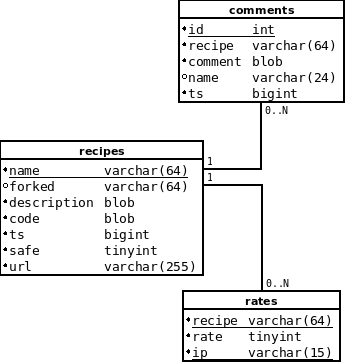
\includegraphics[scale=0.7]{./resources/market_db.png}
  %% \includegraphics[width=0.8\textwidth]{image.png}
  \caption{Schemat bazy danych targowiska}
  \label{fig:awesome_image}
\end{figure}
\section{Serwer}
\section{Moduły systemu - TODelete}
System składa się z biblioteki, przykładowej aplikacji appIFY oraz aplikacji działających na serwerze - Serwera Grup oraz Targowiska.
Aplikacja korzysta z biblioteki oraz komunikuje się z serwerem. Oprócz tego Serwer Grup oraz Targowisko udostępniają z poziomu przeglądarki takie funkcje jak rejestracja użytkowników czy tworzenie Recept.
Miejscem, gdzie zawarta jest główna logika Aplikacji są Recepty -- są w nich opisane wszystkie zdarzenia, które mają nastąpić po spełnieniu pewnych ściśle określonych warunków. Docelowo będą one tworzone przez użytkowników i pobierane z Targowiska, jednak istnieją także przykładowe Recepty wbudowane w Aplikację, mające na celu ułatwienie użytkownikom tworzenia nowych na ich podstawie oraz rozszerzenie początkowej funkcjonalności aplikacji.

\chapter{Opis implementacji}
%% NISKI POZIOM ABSTRAKCJI - detale techniczne - technologie, dokumnetacje, narzędzia, KOD, KOD, jeszcze trochę KODU, jakieś tricki w KODZIE etc.
\section{Użyte technologie}
W tej części zaprezentowano opis technologii użytych bezpośrednio w implementacji składowych platformy.
\subsection{Android}
System operacyjny z rodziny Linux przeznaczony dla urządzeń mobilnych. Aktualnie rozwijane przez sojusz biznesowy Open Handset Alliance.
\subsection{Android SDK}
Platforma programistyczna umożliwiająca tworzenie aplikacji dla systemu Android. Zawiera wtyczkę do środowiska Eclipse, narzędzia wspierające prace programisty, emulator i biblioteki potrzebne do zbudowania aplikacji. Programy dedykowne platformie pisane są w języku Java i uruchamiane na maszynie wirtualnej Dalvik.
\subsection{Apache Commons}
\subsection{Apache HTTP Server}
Otwartoźródłowy serwer HTTP. Najpopularniejsze narzędzie tego typu na świecie. Jego wielką zaletą jest mnogość informacji na jego temat dostępnych w internecie oraz
dostępność na większość znaczących systemów operacyjnych.
\subsection{Git}
Rozproszony oraz wieloplatformowy system kontroli wersji będący wolnym oprogramowaniem. Preferowane narzędzie programistów związanych z otwartym oprogramowaniem.
\subsection{HTML 5}
Język programowania służący do tworzenia współczesnych stron internetowych. Jest rozwinięciem oraz uproszczeniem języka HTML 4.
\subsection{Hibernate}
Narzędzie odwzorowań obiektowo-relacyjnych (ang. object-relation mapping, ORM) rozwijany na zasadzie wolnego oprogramowania. Umożliwia odworowania obiektowo-relacyjne, pamięć podręczną, leniwe (ang. Lazy loading), chciwe pobieranie oraz rozproszoną pamięć podręczną.
\subsection{JSON}
Skrót od JavaScript Object Notation. Jest to lekki, tekstowy format wymiany danych niezależny od języka programowania. Został wybrany ze względu na swoją czytelność i wsparcie ze strony bibliotek programistyzcnych.
\subsection{Java 6}
Jezyk programowania cechujący się obiektowością (ang. Object-oriented programming, OOP) oraz silmnym typowaniem. Kod źródłowy Javy kompilowany jest do kodu bajtowego interpretowanego przez maszynę wirtualną zapewnia to większa niezależność od platformy niż w innych podobnych językach np. C++.
\subsection{JavaScript}
Skryptowy język oprogramowania stosowany na stronach internetowych.
\subsection{Apache Maven}
Narzędzie automatycznego budowania oprogramowania dla języka JAVA. Głównymi problemami jakie rozwiązuje Maven przy budowaniu aplikacji są: zarządzanie zależnościami, mozliwość wieloma modułami, wsparcie dla testów.
\subsection{MySQL}
System zarządzania relacyjnymi bazami danych. Jest to wolne oprogramowanie szczególnie upodobane przez twórców aplikacji internetowych. Bardzo dobrze współpracuje z językami takimi jak PHP czy Java
\subsection{PHP}
Obiektowy język programowania dedykowany generowaniu stron internetowych w czasie rzeczywistym. Szczególnie użyteczny w przypadku tworzenia prototypów tudzież niewielkich projektów wymagających stosunkowo niskiego poziomu abstrakcji.
\subsection{RESTeasy}
Framework oprogramowania służacy do tworzenia aplikacji rozproszonych, oparty na wzorcu architektury oprogramowania Representational State Transfer(REST).
\subsection{SpringFramework}
Framework(Szkielet) tworzenia aplikacji w języku Java a w szczególności JavaEE. Do najważniejszych fukcji Springa zalicza się wstrzykiwanie zależności (ang. dependency injection, DI) oraz programowanie aspektowe (ang. aspect-oriented programming, AOP).  
\subsection{Vaadin}
Framework sieciowy służący do tworzenia aplikacji sieciowych w szczególnosci interfejsu użytkownika w oparciu o Google Web Toolkit (GWT) w języku JAVA.
\subsection{JUnit}
Biblioteka służaca do tworzenia testów jednstkowych w jezyku Java.


\section{Użyte narzędzia}
\subsection{Apache Tomcat}
Kontener aplikacji sieciowych.
\subsection{Eclipse}
Popularne zintegrowane środowisko programistyczne (IDE) wspierające głównie język Java (wtyczki pozwalają obsługiwać inne języki). 
\subsection{Android developer tools}
Wtyczka do Eclipse pozwalająca tworzyć aplikacje androidowe. Dodaje takie funkcjonalności jak edycja plików XML odpowiadających za wygląd aplikacji (również w trybie graficznym) czy debugowanie na telefonach oraz emulatorze.
\subsection{String Tool Suite}
Zintegrowane środowisko programistyczne oparte o Eclipsa dostosowany do SpringFramework.
\subsection{Emacs}
Popularny, w pełni rozszerzalny edytor tekstowy spotykany głównie w systemach operacyjnych z rodziny Unix. Używany przez wysokiej klasy programistów oraz naukowców na całym świecie.
\subsection{Git bash for windows}
Narzędzie umożliwiające używanie Gita z linii poleceń w systemie Windows poprzez wbudowane środowisko MinGW.
\subsection{Github}
Serwis internetowy gromadzący społeczność programistów z całego świata. Służy jako hosting dla otwartoźródłowych projektów zarządzanych za pomocą systemu Git.
Udostępnia szereg narzędzi wspierających - system śledzenia zadań, budowa statystyk.
\subsection{Latex}

\subsection{Linux}
Rodzina systemów operacyjnych będących wolnym oprogramowaniem oraz używajnących jądra Linux.
\subsection{Notepad++}
Prosty edytor tekstowy umożliwiający kolorowanie składni w wielu językach.
\subsection{Przeglądarki internetowe}
Programy takie jak Google Chrome, Mozilla Firefox czy Opera, używane w pracy do testowania rozwiązań mających postać strony internetowej.
\subsection{Windows}
System operacyjny firmy Microsoft.
\section{Użyty sprzęt}
\subsection{Komputery klasy PC}
Podstawowa platforma do wszystkich aspektów pracy, z wyjątkiem testowania, do którego użyliśmy także telefonów.
\subsection{LG Swift GT540}
Procesor: Qualcomm MSM7227 600 MHz
Pamięć RAM: 256 MB
System operacyjny: Android 4.0.1 (Cyanogen mod)
\subsection{Media-Droid IMPERIUS EN3RGY MT7013}
Procesor: dwurdzeniowy, 1GHz ARM7 MTK6577
Pamięć RAM: 256 MB
System operacyjny: Android 4.1.2
\subsection{Motorola Defy MB525}
Procesor: TI OMAP3610 800 MHz
Pamięć RAM: 512 MB
System operacyjny: Android 4.3.1 (Cyanogen mod)
\subsection{Sony LT18 Xperia Arc S}
Procesor: Qualcomm MSM8255T 1,40 GHz
Pamięć RAM: 512 MB
System operacyjny: Android 4.0.4
\subsection{Samsung Galaxy Mini GT-S5570}
Procesor: Qualcomm MSM7227 600 MHz
Pamięć RAM: 384 MB
System operacyjny: Android 2.2
\section{Recepty}
\section{Biblioteka}
\section{Aplikacja kliencka}
\subsection{Moduł obsługi recept}
\subsection{Moduły dostępu do systemu}
\section{Targowisko}
\section{Serwer}
\subsection{Repozytorium recept}
\subsection{Serwer recept grupowych}
\section{Protokół komunikacji}
Komunikacja aplikacji klienckich oparta jest o ciagłe odpytywanie (ang. polling). 
Wymiana danych odbywa się przy użyciu tekstowego formatu danych JSON. 

\section{Opis pakietów}
\subsection{Pakiety Aplikacji}
pl.poznan.put.cs.ify.app - główny pakiet Aplikacji.
pl.poznan.put.cs.ify.jars - pakiet odpowiedzialny za zarządzanie plikami .jar zawierającymii recepty pobrane z Targowiska.
pl.poznan.put.cs.ify.core - pakiet odpowiedzialny za zarządzanie dostępnymi i aktywowanymi Receptami.
pl.poznan.put.cs.ify.appify.receipts - pakiet zawierający Recepty wbudowane w Aplikację.
pl.poznan.put.cs.ify.app.ui - pakiet zawierający kontrolki interfejsu użytkownik.
pl.poznan.put.cs.ify.app.ui.params - pakiet zawierający kontrolki interfejsu użytkownika wykorzystywane do wprowadzania parametrów przy inicjalizacji Recepty.
pl.poznan.put.cs.ify.app.market - pakiet odpowiedzialny za pobieranie danych z Targowiska i wyświetlanie ich.
pl.poznan.put.cs.ify.app.fragments - pakiet zawierający widoki ekranów aplikacji.
\subsection{Pakiety Biblioteki}
pl.poznan.put.cs.ify.api - pakiet główny Biblioteki.
pl.poznan.put.cs.ify.api.exceptions - pakiet zawierający wyjątki, które mogą być rzucane przez metody z Biblioteki.
pl.poznan.put.cs.ify.api.features - pakiet zawietający Podfunkcjonalności i Zdarzenia.
pl.poznan.put.cs.ify.api.group - pakiet odpowiedzialny za obsługę Recept Grupowych.
pl.poznan.put.cs.ify.api.log - pakiet odpowiedzialny za obsługę logowania i domyślny widok logów.
pl.poznan.put.cs.ify.api.params - pakiet zawierający typy parametrów wykorzystywanych przez Recepty.
pl.poznan.put.cs.ify.api.security - pakiet odpowiedzialny za moduł uprawnień Biblioteki.
pl.poznan.put.cs.ify.api.types - pakiet zawierający typy danych wykorzystywanych przez Biblioteke.
\subsection{Pakiety Serwera}
pl.poznan.put.cs.ify.webify - pakiet główny serwera.
pl.poznan.put.cs.ify.webify.data.dao - pakiet zawierający warstwe dostępu do danych.
pl.poznan.put.cs.ify.webify.data.entity - pakiet zawierający klasy odwzorowywane na bazę danych.
pl.poznan.put.cs.ify.webify.data.enums - pakiet zawierajacy potrzebne w bazie danych typy wyliczeniowe(np. lista ról). 
pl.poznan.put.cs.ify.webify.gui - pakiet główny graficznego interfejsu użytkownika.
pl.poznan.put.cs.ify.webify.gui.windows - paiet zawierający wszytskie okna aplikacji sieciowej.
pl.poznan.put.cs.ify.webify.gui.components - pakiet zawierający komponenty użyte w aplikacji.
pl.poznan.put.cs.ify.webify.gui.session - 
pl.poznan.put.cs.ify.webify.service - pakiet zawierający logikę.
pl.poznan.put.cs.ify.webify.rest - pakiet zawerajacy obsługę zapytań typu REST.
pl.poznan.put.cs.ify.webify.utils - pakiet, w którym przechowywane są funkcje pomocnicze używane w całym projkcie.

\chapter{Testy oraz wyniki?}
%% jeszcze tego nie wiem, ale to będzie niejako wstęp do zakończenia
\chapter{Zakończenie}
% ostateczne podsumowanie uzyskanych wyników + ew. wybieganie w przyszłość, marzenia i inne bajanie w obłokach

\appendix

\chapter{Przewodnik użytkownika}
\section{Opis Podfunkcjonalności}
\subsection{Akcelerometr (YAccelerometerFeature.java)}
Umożliwia reagowanie na odczyty akcelerometru wbudowanego w urządzenie. 

\subsection{Battery (YBatteryFeature.java)}
Umożliwia reagowanie na zmiany poziomu baterii urządzenia.

\subsection{SMS (YSMSFeature.java)}
Umożliwia wysyłanie wiadomości SMS oraz reagowanie na wiadomości przychodzące.

\subsection{Wifi (YWifiFeature.java)}
Umożliwia włączanie i wyłączanie modułu WiFi urządzenia.

\subsection{GPS (YGPSFeature.java)}
Umożliwa śledzenie pozycji urządzenia za pomocą modułu GPS.

\subsection{Sound (YSoundFeature.java)}
Pozwala odtrzarzać pliki dźwiękowe.

\subsection{RawPlayer (YRawPlayerFeature.java)}

\subsection{Group (YGroupFeature.java)}

\subsection{Geocoder (YGeocoderFeature.java)}
Umożliwia pobranie adresu związanego z podaną długościa i szerokością geograficzną.

\subsection{Time (YTimeFeature.java)}

\subsection{AudioManager (YAudioManager.java)}

\subsection{Text (YTextFeature.java)}

\subsection{Internet (YInternetFeature.java)}
Umożliwia wysyłanie i pobieranie danych z podanego adresu.

\subsection{Calls (YCallsFeature.java)}
Umożliwia reagowanie na połączenia przychodzące i inicjowanie połączeń wychodzących.

\subsection{Notification (YNotificationFeature.java)}
Umożliwia wyświetlanie powiadomień w interfejsie graficznym urządzenia.

\backmatter

\begin{thebibliography}{1}
%Jak się używa jednej ksiązki to jest plagiat ale jak wielu to jest poprostu bibliografia.
\bibitem{onx}Projekt on\{X\} http://www.onx.ms/\#!findOutMorePage. Ostatnio odwiedzone 6/02/13.
\bibitem{springinaction}C.~Walls. \emph{Spring in action, 3rd edition}. Manning Publication Co, 2011.
\bibitem{vaadinbook}Vaadin https://vaadin.com/book/vaadin6/-/page/preface.html 
\bibitem{patterns}E.~Gamma. \emph{Design Patterns, First edition}. Person Education, Inc, 1995.
\end{thebibliography}

\end{document}
